\newcommand{\hmwkTitle}{Homework 9}
\newcommand{\hmwkDueDate}{Tuesday, March 24, 2026}
\newcommand{\hmwkHeaderTitle}{ICCS206 Discrete Mathematic: Homework 9}
\documentclass{article}

\usepackage{fancyhdr}
\usepackage{amsmath}
\allowdisplaybreaks
\usepackage{amsthm}
\usepackage{amsfonts}
\usepackage{tikz}
\usepackage[plain]{algorithm}
\usepackage{algpseudocode}
\usepackage{enumitem}
\usepackage{graphicx}
\usepackage{hyperref}

\usetikzlibrary{automata,positioning}

%
% Basic Document Settings
%

\topmargin=-0.45in
\evensidemargin=0in
\oddsidemargin=0in
\textwidth=6.5in
\textheight=9.0in
\headsep=0.25in

\linespread{1.1}

\pagestyle{fancy}
\lhead{\hmwkAuthorName}
\chead{} % empty
\rhead{\hmwkHeaderTitle}
\cfoot{\thepage}

\renewcommand\headrulewidth{0.4pt}
\renewcommand\footrulewidth{0pt}

\setlength\parindent{0pt}

%
% Homework Details
%

\providecommand{\hmwkTitle}{Homework}
\providecommand{\hmwkDueDate}{TBD}
\providecommand{\hmwkClass}{ICCS206 Discrete Mathematic}
\providecommand{\hmwkClassTime}{Section\ 1}
\providecommand{\hmwkClassInstructor}{Pakawut Jiradilok}
\providecommand{\hmwkAuthorName}{\textbf{Jiraroj Wiruchpongsanon (6781617)}}
\providecommand{\hmwkHeaderTitle}{\hmwkClass:\ \hmwkTitle}

%
% Title Page
%

\title{
    \vspace{2in}
    \textmd{\textbf{\hmwkClass:\ \hmwkTitle}}\\
    \normalsize\vspace{0.1in}\small{Due\ on\ \hmwkDueDate}\\
    \vspace{0.1in}\large{\textit{\hmwkClassInstructor\ \hmwkClassTime}}
    \vspace{3in}
}

\author{\hmwkAuthorName}
\date{}

\renewcommand{\part}[1]{\textbf{\large Part \Alph{partCounter}}\stepcounter{partCounter}\\}

%
% Helper Commands
%

\newcounter{partCounter}
\newcommand{\solution}{\textbf{\large Solution}}

\newtheorem*{theorem}{Theorem}

\theoremstyle{remark}
\newtheorem*{remark}{Remark}

\begin{document}

\maketitle
\newpage


\usepackage{tikz}
\usetikzlibrary{matrix}

\section*{Problem 1: Minesweeper Theorem}
Given any rectangular Minesweeper board, show that the sum of all hint numbers equals the sum of all hint numbers on the complement board (bombs and empty cells swapped).

\medksip
\solution

using the given minesweeper configuration as an example, 

\begin{figure}[h]
    \centering

    \begin{minipage}{0.45\textwidth}
        \centering
        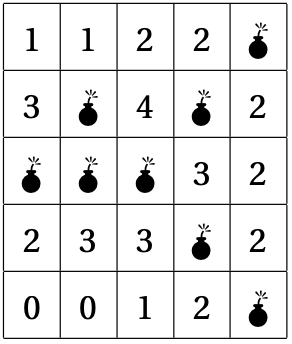
\includegraphics[height=4cm]{HW9_minesweeper1.png}
    \end{minipage}
    \hfill
    \begin{minipage}{0.45\textwidth}
        \centering
        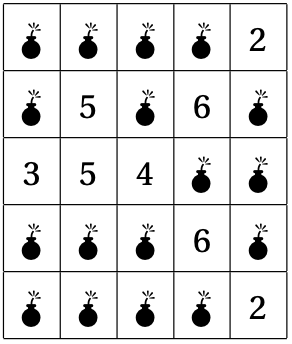
\includegraphics[height=4cm]{HW9_minesweeper2.png}
    \end{minipage}

\end{figure}

we'll see that the summation of mines indication numbers are the same on the first configuration and it's reversed counter-part, equals to 33. 

\vspace{1em}


as the indication numbers are directly ties to the bomb (no relation to adjacent nodes of the same kind), we can write the first configuration as a graph as

\begin{center}
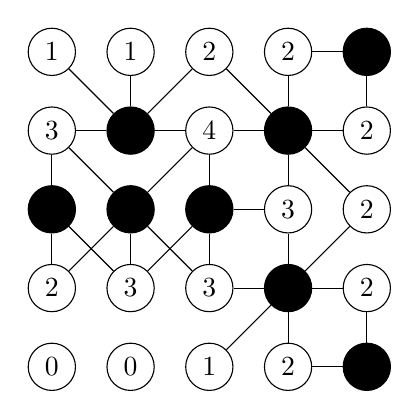
\begin{tikzpicture}
\tikzset{
    v/.style={circle, draw, minimum size=6mm, inner sep=0pt},
    blackv/.style={circle, draw, fill=black, minimum size=6mm, inner sep=0pt}
}

% --- nodes ---
\node[v] (v11) at (1,-1) {1};
\node[v] (v12) at (2,-1) {1};
\node[v] (v13) at (3,-1) {2};
\node[v] (v14) at (4,-1) {2};
\node[blackv] (v15) at (5,-1) {};

\node[v] (v21) at (1,-2) {3};
\node[blackv] (v22) at (2,-2) {};
\node[v] (v23) at (3,-2) {4};
\node[blackv] (v24) at (4,-2) {};
\node[v] (v25) at (5,-2) {2};

\node[blackv] (v31) at (1,-3) {};
\node[blackv] (v32) at (2,-3) {};
\node[blackv] (v33) at (3,-3) {};
\node[v] (v34) at (4,-3) {3};
\node[v] (v35) at (5,-3) {2};

\node[v] (v41) at (1,-4) {2};
\node[v] (v42) at (2,-4) {3};
\node[v] (v43) at (3,-4) {3};
\node[blackv] (v44) at (4,-4) {};
\node[v] (v45) at (5,-4) {2};

\node[v] (v51) at (1,-5) {0};
\node[v] (v52) at (2,-5) {0};
\node[v] (v53) at (3,-5) {1};
\node[v] (v54) at (4,-5) {2};
\node[blackv] (v55) at (5,-5) {};

% --- edges (horizontal) ---
\draw (v14)--(v15);
\draw (v21)--(v22) (v22)--(v23) (v23)--(v24) (v24)--(v25);
\draw (v33)--(v34);
\draw (v43)--(v44) (v44)--(v45);
\draw (v54)--(v55);

% --- edges (vertical) ---
\draw (v21)--(v31) (v31)--(v41);
\draw (v12)--(v22) (v32)--(v42);
\draw (v23)--(v33) (v33)--(v43);
\draw (v14)--(v24) (v24)--(v34) (v34)--(v44) (v44)--(v54);
\draw (v15)--(v25)(v45)--(v55);

% --- edges (diagonal down-right) ---
\draw (v11)--(v22) (v13)--(v24);
\draw (v21)--(v32) (v24)--(v35);
\draw (v31)--(v42) (v32)--(v43);

% --- edges (diagonal down-left) ---
\draw (v13)--(v22);
\draw (v23)--(v32);
\draw (v32)--(v41) (v33)--(v42) (v35)--(v44);
\draw (v44)--(v53);
\end{tikzpicture}
\end{center}

\vspace{1em}
\hrulefill

\section*{Problem 2: Graph Isomorphism}
For the three graphs $G_1$, $G_2$, $G_3$ below determine which pairs, if any, are isomorphic. For each isomorphic pair provide an explicit isomorphism; otherwise briefly justify why they are not isomorphic.

\begin{figure}[h]
    \centering
    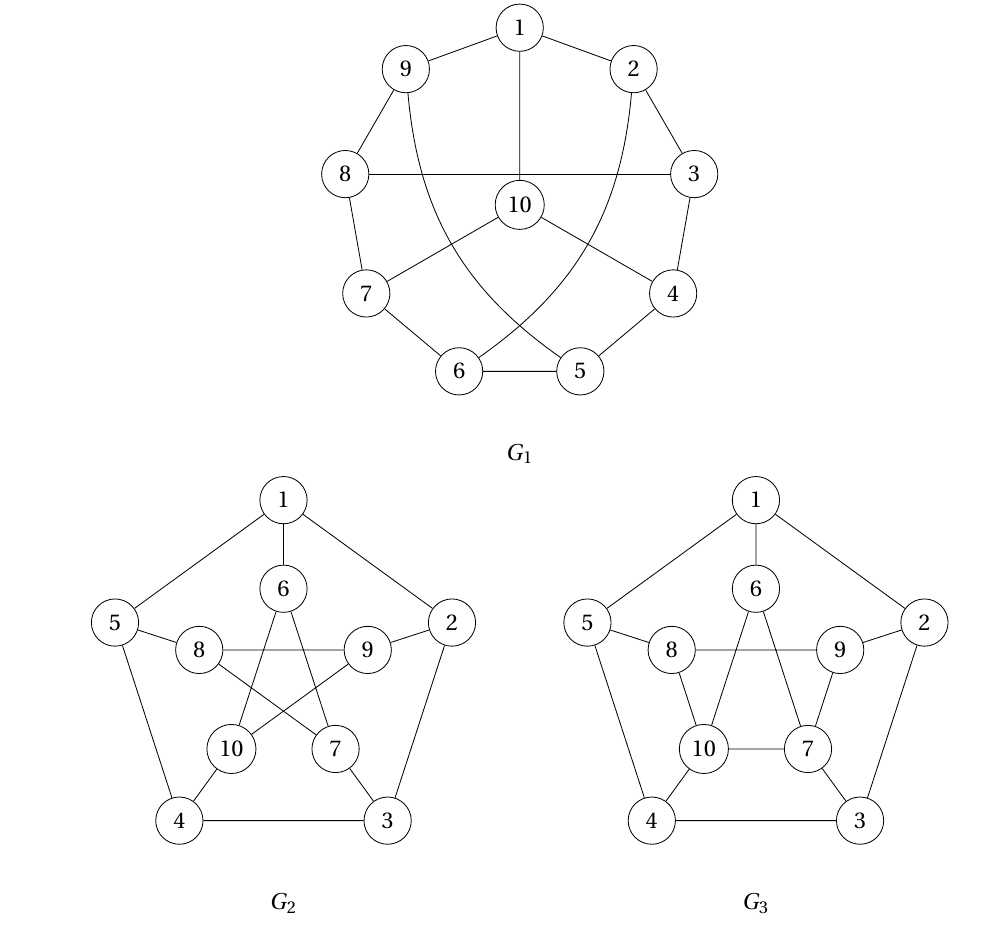
\includegraphics[width=0.8\textwidth]{HW9_graphs.png}
\end{figure}

\section*{Problem 3: Meeting Scheduler}
We need to schedule executive meetings without conflicts (each person attends at most one meeting at a time). Each meeting lasts one hour.
\[
\begin{array}{c|l}
\text{Meeting} & \text{Members} \\
\hline
A & \{ \text{Smith, Jones, Brown, Green} \} \\
B & \{ \text{Jones, Wagner, Chase} \} \\
C & \{ \text{Harris, Oliver} \} \\
D & \{ \text{Harris, Jones, Mason} \} \\
E & \{ \text{Oliver, Cummings, Larson} \}
\end{array}
\]
What is the minimum number of hours needed and how should the meetings be scheduled?

\section*{Problem 4: DNA Sequence}
Shotgun sequencing produced the subsequences $\{\text{CAT}, \text{TCA}, \text{AAG}, \text{GCT}, \text{GCA}, \text{ATC}, \text{CAA}, \text{AGC}\}$.
What is the original sequence?

\section*{Problem 5: Yoyo Distribution Network}
As CEO you must ship yoyos between distribution centers at minimum total cost. The network and edge costs are shown below (note $AC$ costs $2$, $AD$ costs $1$, and $EB$ costs $3$). Find the optimal routing plan.
\begin{center}
    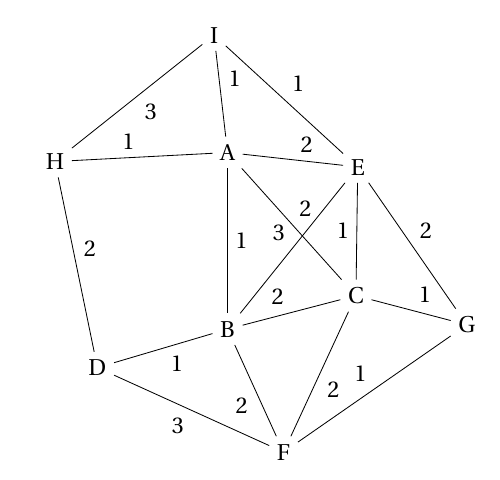
\includegraphics[width=0.5\textwidth]{HW9_network.png}
\end{center}

\section*{Problem 6: One-Stroke Game}
For each graph below determine whether it can be drawn in one stroke (an Euler trail). If so, exhibit the stroke order; otherwise explain why it is impossible.
\begin{center}
    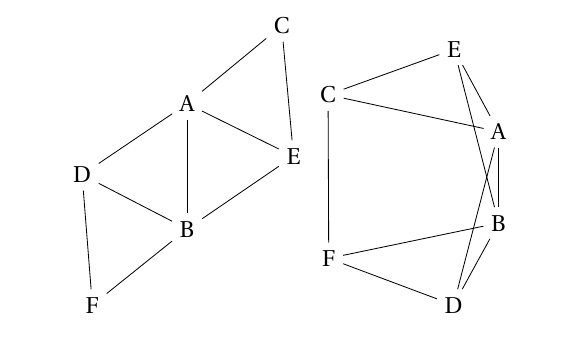
\includegraphics[width=0.45\textwidth]{HW9_onestroke.png}
\end{center}

\end{document}
